\Chapter{\textit{Design} de Testes Economicamente Viáveis}

Tradução de Élisson Michael Fernandes Meirelles Araújo. Disponível em: \url{github.com/elissonmichael/design-de-testes-economicamente-viaveis}

\cite{Sandi} afirma que escrever código que muda é uma arte a qual a prática depende de três habilidades diferentes.

Primeiro, você precisa entender \textit{design} orientado a objetos. Código com \textit{design} pobre é naturalmente difícil de alterar. De um ponto de vista prático, a capacidade de alteração é a única métrica de \textit{design} que importa; código que é fácil de mudar tem um bom \textit{design}. Se você chegou até aqui é justo supor que você já tem uma base pela qual começar a praticar a escrita de código fácil de alterar.

Segundo, você deve ser habilidoso em refatoração de código. Não no sentido casual de "vá até a sua aplicação e tire algumas coisas", mas no sentido real, maduro, à prova de balas definido por Martin Fowler no livro \textit{Refactoring: Improving the Design of Existing Code}\cite{Fowler1999}:

\say{Refatoração é o processo de mudar um sistema de software de um modo que não altere o comportamento externo do código, mas melhore a estrutura interna.}

Repare na parte \textit{não altere o comportamento externo do código}. Refatorar, em sua definição formal, não adiciona novo comportamento, ele melhora a estrutura existente. É um processo preciso que altera código via passos muito pequenos, cuidadosos, incrementais que infalivelmente transforma um \textit{design} em outro.

Bom \textit{design} preserva flexibilidade máxima no menor custo ao adiar decisões a cada oportunidade. Postergando qualquer comprometimento até que requerimentos mais específicos cheguem. Quando esse dia chegar, será através da refatoração que você vai transformar a estrutura atual do código em uma que acomodará os novos requerimentos. Novas \textit{features} serão adicionadas apenas depois que tiver refatorado o código com sucesso.

Se as suas habilidades de refatorar são fracas, melhore-as. A necessidade de  \textit{refactoring} contínuo é uma consequência natural do bom \textit{design}; seus esforços para melhorar o \textit{design} irão dar seu maior retorno apenas quando você refatorar com facilidade.

Para finalizar, a arte de escrever código mutável requer a habilidade de escrever testes que tenham valor. Testes te dão confiança para refatorar constantemente. Testes eficientes provam que o código alterado continua se comportando corretamente sem aumentar os custos no geral. Bons testes são escritos de uma forma que a alteração do código não force a reescrita dos testes, permitindo que refatorações possam ser realizadas sem medo e insegurança.

A escrita de testes que executem este truque é um questão de \textit{design} e é o tópico desse capítulo.

Uma compreensão de \textit{design} orientado a objetos, boas habilidades de refatoração e a habilidade de escrever testes eficientes formam a base principal onde reside o código de alteração fácil.

Código com bom \textit{design} é fácil de alterar, \textit{refactoring} é como você muda de um \textit{design} para o próximo e testes te libertam para refatorar de forma impune.

\section{Testando Intencionalmente}

Os argumentos mais comuns a favor de se ter testes é o de que eles reduzem \textit{bugs}, fornecem documentação e que escrever testes primeiro melhora o \textit{design} da aplicação.

Esses benefícios, apesar de válidos, são representações para um objetivo mais profundo. O verdadeiro propósito de testar, assim como o verdadeiro propósito do \textit{design}, é a redução de custos. Se escrever, manter e executar testes consome mais tempo do que seria necessário para corrigir \textit{bugs}, escrever documentação e fazer o \textit{design} de aplicações, testes claramente não valem a pena serem escritos e nenhuma pessoa racional iria contradizer isso.

É comum para programadores que são novos em testes encontrarem-se em um estado infeliz onde os testes que eles escrevem custam mais do que o valor que esses testes promovem, e que assim sendo querem discutir sobre o valor de se testar. Esses são programadores os quais acreditam serem altamente produtivos em suas formas sem testes, pois são os mesmos que bateram na parede to testar primeiro e tropeçaram até parar. Suas tentativas em programação com testes primeiro resultaram em menos entregas, e o desejo de retornar a serem produtivos fizeram com que eles retornassem aos antigos hábitos e esquecessem a escrita de testes.

A solução para o problema de testes custosos, no entanto, não é parar de testar, mas se tornar melhor nisso. Obter um bom retorno dos testes requer clareza de intenção e saber o que, quando e como testar.

\section{Conhecendo as suas Intenções}

Testar tem muito benefícios em potencial, alguns óbvios, outros mais obscuros. Uma compreensão completa desses benefícios vai aumentar a sua motivação para alcança-los.

\subsection{Encontrando \textit{bugs}}

Encontrar falhas, ou \textit{bugs}, cedo no processo de desenvolvimento rendem grandes dividendos. Não apenas é mais fácil encontrar e corrigir um \textit{bug} quanto mais próximo da sua época de criação, mas conseguir o código certo mais cedo do que mais tarde pode ter um efeito positivo não esperado no \textit{design} resultante.

Saber que você pode (ou não pode) fazer algo mais cedo talvez façam você escolher alternativas no dia presente que alteram as opções de \textit{design} disponíveis no futuro. Além disso, conforme o código se acumula, \textit{bugs} incorporados acumulam dependências. Corrigir esses \textit{bugs} mais tarde no processo pode necessitar da mudança de muito código com dependências. Corrigir esses \textit{bugs} mais cedo sempre custa menos.

\subsection{Fornecimento de Documentação}

Testes providenciam a única documentação confiável de \textit{design}. A história que eles contam permanecem verdadeiras muito tempo depois que a documentos em papel se tornam obsoletos e a memória humana falha. Escreva seus testes como se você esperasse que o seu futuro eu tenha amnésia. Lembre-se que você vai esquecer; escreva testes que te lembrem da história que uma vez você viveu.

\subsection{Adiando Decisões de \textit{Design}}

Testes permitem que você adie de forma segura decisões de \textit{design}. Conforme as suas habilidades de \textit{design} melhoram você vai começar a escrever aplicações que estão semeadas com lugares onde você sabe que o \textit{design} precisa de alguma coisa, mas você não tem ainda informações suficientes para saber exatamente o que. Esses são os lugares onde você está aguardando informações adicionais, resistindo de forma valente as forças que obrigam você a se cometer a um \textit{design} específico.

Esses pontos de decisão ''pendente'' são frequentemente codificados como \textit{hacks} concretos levemente embaraçosos escondidos atrás de interfaces totalmente apresentáveis. Essa situação ocorre quando você está ciente de um caso concreto no presente, mas você espera totalmente que novos casos chegarão em um futuro próximo. Você sabe que em algum ponto você vai estar melhor servido por código que controla melhor esses muitos casos concretos em uma única abstração, mas exatamente agora você não tem informação suficiente para antecipar qual será essa abstração.

Quando seus testes dependem de interfaces você pode refatorar o código por baixo com total desapego. Os testes verificam a continuação do bom comportamento da interface e mudanças no código subjacente não forçam a reescrita dos testes. Depender intencionalmente em interfaces permite que você use testes para postergar decisões de \textit{design} com segurança e sem penalidade alguma.

\subsection{Suporte para Abstrações}

Quando mais informações finalmente chegarem e você tomar a próxima decisão de \textit{design}, você vai alterar o código de maneiras que aumentem seu nível de abstração. Onde mora outros benefícios de testes no \textit{design}.

Bom \textit{design} naturalmente progride em direção a pequenos objetos independentes que dependem de abstrações. O comportamento de aplicações com bom \textit{design} gradualmente são o resultado de interações entre essas abstrações. Abstrações são componentes de \textit{design} maravilhosamente flexíveis, mas as melhorias que eles fornecem vêm com um pequeno custo: Enquanto cada abstração possa ser fácil de entender individualmente, não há um único local no código que torne óbvio o comportamento do todo.

Conforme a base de código cresce e o número de abstrações aumenta, testes se tornam cada vez mais necessários. Há um nível de abstração em \textit{design} onde é quase impossível fazer qualquer alteração de forma segura a menos que o código tenha testes. Testes são os registros das interfaces de cada abstração e como tal eles são a sua proteção. Eles permitem que você adie decisões de \textit{design} e crie abstrações em qualquer nível de profundidade útil.

\subsection{Expondo Falhas de \textit{Design}}

O próximo benefício de testes é que eles expõem falhas de \textit{design} no código subjacente. Se um teste requer um configuração trabalhosa, o código espera muito contexto. Se testar um objeto traz um monte de outros objetos, o código tem muitas dependências. Se o teste é difícil de escrever, outro objetos irão achar difícil reutilizar o código.

Quando o \textit{design} é ruim, testar é difícil. No entanto, não é garantido que o inverso seja verdade. Testes custosos não necessariamente significam que a aplicação tem \textit{design} pobre. É tecnicamente possível escrever testes ruins para código com bom \textit{design}. Assim sendo, para testes diminuírem seus custos, tanto a aplicação subjacente e os testes precisam ter bom \textit{design}.

Seu objetivo é ganhar todos os benefícios dos testes pelo menor custo possível. O melhor jeito de alcançar esse objetivo é escrever testes fracamente acoplados apenas sobre as coisas que importam.

\section{Sabendo o que Testar}

A maioria dos programadores escrevem testes demais. Isso não é sempre óbvio porque em muitos casos o custo desses testes desnecessários são tão altos que os programadores envolvidos já desistiram de testar completamente. Não é que eles não têm testes. Eles têm uma grande, mas obsoleta suíte de testes, que nunca roda. Um jeito simples de obter melhores utilidades dos testes é escrever menos deles. O jeito mais seguro de conseguir isso é testar tudo apenas uma vez e no lugar certo.

Remover duplicação de testes diminui o custo da mudança de testes quando há mudanças na aplicação, e colocar testes nos lugares certos garantem que eles serão forçados a mudar apenas quando absolutamente necessário. Refinar seus testes para apenas o essencial requer ter uma ideia muito clara sobre o que você pretende testar, uma que pode ser derivada de princípios de \textit{design} que você já conhece.

Pense em uma aplicação orientada a objetos como uma série de mensagens passando entre um conjunto de caixas pretas. Lidar com cada objeto como se fosse uma caixa preta restringe o que outros tem permissão para saber e limita o conhecimento público sobre qualquer mensagens que atravessam suas fronteiras.

Objetos com bom \textit{design} têm fronteiras que são fortes. Cada um é como a cápsula espacial exibida na Figura \ref{img:origem_mensagens}. Nada no exterior pode ver dentro, nada dentro pode ver o exterior e apenas algumas mensagens explicitamente acordadas podem passar pelas fechaduras.

\begin{figure}[!htbp]
  \center
  \includegraphics[scale=0.40]{imagens/origem_mensagens.png}
  \caption{Objetos em teste são como cápsulas espaciais, mensagens abrem suas brechas}
  \label{img:origem_mensagens}
\end{figure}

Essa ignorância da parte interna de todos os outros objetos é a parte central do \textit{design}. Lidar com objetos como se eles fossem apenas e exatamente as mensagens as quais eles respondem permite que você faça o \textit{design} de uma aplicação que é alterável, e é o seu entendimento sobre a importância dessa perspectiva que vai permitir que você crie testes que fornecem o máximo de benefício com o mínimo de custo.

Os princípios de \textit{design} que você está impondo a sua aplicação também se aplicam aos seus testes. Cada teste é meramente outro objeto da aplicação que precisa usar uma classe existente. Quanto mais o teste fica acoplado aquela classe, mais emaranhado os dois se tornam e mais vulnerável o teste se torna a ser forçado a mudar desnecessariamente.

Não apenas você deveria limitar o acoplamento, mas os poucos que você permite deveriam ser a coisas estáveis. A coisa mais estável sobre qualquer objeto é a sua interface pública; segue-se logicamente que os testes que você escreve devem ser para mensagens que são definidas nas interfaces públicas. Os testes mais custosos e inúteis são aqueles que abrem um buraco nas paredes de contenção de um objeto ao se acoplarem a detalhes internos instáveis. Esses testes ansiosos provam nada sobre exatidão no geral de uma aplicação, mas no entanto aumentam custos porque eles quebram a cada refatoração da classe por baixo.

Testes deveriam se concentrar nas mensagens de entrada e saída que cruzam as fronteiras do objeto. As mensagens de entrada compõem a interface pública do objeto que recebe. As mensagens de saída, por definição, são entradas para outros objetos e então são parte da interface de algum outro objeto, como ilustrado na Figura \ref{img:dependencia}.

\begin{figure}[!htbp]
  \center
  \includegraphics[scale=0.40]{imagens/dependencia.png}
  \caption{Uma mensagem de saída de um objeto é a mensagem de entrada de outro objeto}
  \label{img:dependencia}
\end{figure}

Na Figura \ref{img:dependencia}, mensagens que são entrada em Foo compõem a interface pública de Foo. Foo é responsável por testar sua própria interface e faz isso ao fazer afirmações (\textit{assertions}) sobre os resultados que essas mensagens retornam. Testes que fazem afirmações sobre os valores que as mensagens retornam são testes de \textit{estado}. Testes assim comumente afirmam que os resultados retornados por uma mensagem são iguais a um valor esperado.

A Figura \ref{img:dependencia} também mostra Foo enviando mensagens para Bar. Uma mensagem enviada de Foo para Bar é uma mensagem de saída para Foo, mas uma mensagem de entrada para Bar. Essa mensagem é parte da interface pública de Bar e portanto todos os testes de estado devem então estarem confinados em Bar. Foo não precisa, nem deve, testar o estado dessas mensagens de saída. A regra geral é que objetos devem fazer afirmações sobre o estado apenas das mensagens de suas próprias interfaces públicas. Seguir essa regra limita os testes de retorno de valores de mensagens a apenas um lugar e remove duplicações desnecessárias, fazendo com que seus testes fiquem DRY (\textit{Don't Repeat Yourself}) e reduzindo custos de manutenção.

O fato de você não precisar testar o estado de mensagens de saída não significa que mensagens de saída não precisam de teste algum. Existem dois sabores de mensagens de saída, e um deles requer um tipo diferente de teste.

Algumas mensagens de saída não têm efeito colateral e portanto importam apenas para quem as envia. Quem envia a mensagem com certeza se importa com o resultado que obtém como retorno (por que outro motivo enviar uma mensagem?), mas nenhuma outra parte da aplicação se importa se a mensagem é enviada. Mensagens de saída como essa são conhecidas como \textit{queries} (consultas) e elas não precisam ser testadas pelo objeto que envia a mensagem. Mensagens de consulta são parte da interface pública do objeto que as recebe, o qual já implementa todos os testes de estado necessários.

Contudo, muitas mensagens de saída têm efeitos colaterais (um arquivo é escrito, um registro no banco de dados é salvado, uma ação é tomada por um observador) sobre os quais sua aplicação depende. Essas mensagens são comandos e é responsabilidade do objeto que as envia provar que essas mensagens estão sendo enviadas de forma apropriada. Provar que uma mensagem é enviada é um teste de comportamento, não estado, e envolve afirmações sobre o número de vezes, e com quais argumentos, a mensagem é enviada.

Aqui, então, estão as diretrizes sobre o que testar: Mensagens de entrada devem ser testadas pelo estado que retornam. Mensagens de comando de saída devem ser testadas para certificar que elas são enviadas. Mensagens de saída de consulta não devem ser testadas.

Enquanto os objetos da sua aplicação lidem uns com os outros estritamente via interface pública, seus testes não precisam saber de nada mais. Quando você testa esse conjunto mínimo de mensagens, nenhuma mudança no comportamento privado de qualquer objeto pode afetar nenhum teste. Quando você testa mensagens de comando de saída apenas para provar que elas são enviadas, seus testes fracamente acoplados podem tolerar mudanças na aplicação sem serem forçados a mudar por sua vez. Enquanto as interfaces públicas permanecerem estáveis, você pode escrever testes uma vez e eles irão manter você seguro para sempre.

\section{Sabendo Quando Testar}

Você deve escrever testes primeiro, sempre que faça sentido fazer isso dessa forma.

Infelizmente, julgar quando isso faz sentido pode ser um desafio para \textit{designers} novatos, o que torna esse conselho menos do que útil. Novatos frequentemente escrevem código que é muito acoplado; eles combinam responsabilidades sem relação e vinculam muitas dependências em todos os objetos. Suas aplicações são tapeçarias bem tecidas de código emaranhado onde nenhum objeto vive em isolação. É muito difícil de testar essas aplicações retroativamente porque testes são reuso e esse código não pode ser reutilizado.

Escrever testes primeiro força que um mínimo de reutilização seja construído no objeto durante seu princípio; seria impossível de outra forma escrever qualquer teste. Assim sendo, \textit{designers} novatos são melhores servidos escrevendo código de testes primeiro. A falta de habilidade de \textit{design} deles talvez torne isso desconcertantemente difícil, mas se eles persistirem eles terão pelo menos código testável, algo que de outra forma não seria verdade.

Esteja avisado, no entanto, que escrever testes primeiro não é substituto para e não garante uma aplicação com bom \textit{design}. A reusabilidade que resulta dos testes primeiro é uma melhoria em relação a nenhum teste, mas a aplicação resultante ainda pode cair longe de ter bom \textit{design}. Novatos bem intencionados frequentemente escrevem testes caros e duplicados ao redor de código fortemente acoplado e bagunçado. É uma verdade lamentável que o código mais complexo é geralmente escrito pela pessoa menos qualificada. Isso não reflete uma complexidade natural da tarefa por baixo, mas uma falta de experiência por parte do programador ao invés. Programadores novatos ainda não têm as habilidades para escrever código simples.

As aplicações super complicadas que estes novatos produzem deveriam ser vistas como triunfos da perseverança; é um milagre que essas aplicações funcionem no fim das contas. O código é difícil. As aplicações são difíceis de mudar e cada refatoração quebra todos os testes. Esse custo alto de mudança pode facilmente iniciar um queda de produtividade que pode desanimar todos os interessados. Mudanças desencadeiam efeitos colaterais em cascata ao longo da aplicação, e o custo de manutenção dos testes fazem com que eles pareçam custosos em relação ao valor deles.

Se você é um novato nessa situação, é importante manter a confiança no valor dos testes. Realizada no tempo certo e na quantidade certa, testar, e escrever código de testes primeiro, irá diminuir seus custos no geral. Ganhar esses benefícios requer a aplicação dos princípios de \textit{design} orientado a objetos em todos os lugares, tanto no código da aplicação quanto no código dos seus testes. Seu conhecimento recém-descoberto de \textit{design} já torna mais fácil escrever código testável, a maior parte do restante desse capítulo ilustra como aplicar esses princípios de \textit{design} durante a construção de testes. Pela razão de aplicações com bom \textit{design} serem fáceis de mudar, e teste com bom \textit{design} possivelmente evitarem mudança completamente, essas melhorias de \textit{design} no geral pagam tudo dramaticamente.

\textit{Designers} experientes colhem melhorias mais sutis da escrita de testes primeiro. Não é que eles não conseguem se beneficiar com isso ou que eles nunca vão descobrir algo inesperado ao seguir o que isso dita, em vez disso os ganhos acumulados da reutilização forçada de código são aqueles que eles já possuem. Esses programadores já escrevem código reutilizável fracamente acoplado; testes adicionam valores de outras formas.

Não é inédito para \textit{designers} experientes explorarem soluções para um problema, ou seja, escrever códigos que são apenas experimentos. Esses experimentos são exploratórios, para soluções incertas de alguns problemas. Uma vez que a clareza é obtida e o \textit{design} se sugere, esses programadores então regressam para a escrita de código de produção com testes primeiro.

Seu objetivo geral é a criação de aplicações com bom \textit{design} que possuem cobertura de testes aceitáveis. O melhor jeito de alcançar essa meta varia de acordo com a experiência e pontos fortes do programador.

Essa licença para usar o seu próprio julgamento não é uma permissão para pular os testes. Código com \textit{design} pobre sem testes é apenas código legado que não pode ser testado. Não superestime seus pontos fortes e use um visão inflada de si mesmo como desculpas para evitar testes. Enquanto algumas vezes faz sentido escrever um pouco de código da maneira antiga, você deveria errar ao lado de testes primeiro.

\section{Sabendo Como Testar}

Qualquer um pode criar um novo \textit{framework} de testes em Ruby e algumas vezes parece que todo mundo já criou. O brilhante \textit{framework} novo pode conter uma \textit{feature} que você simplesmente não pode viver sem; se você entende os custos e benefícios, sinta-se livre para escolher qualquer \textit{framework} que sirva para você.

No entanto, há muitas boas razões para ficar dentro das convenções ao testar. Os \textit{frameworks} mais utilizados têm o melhor suporte. Eles são atualizados rapidamente para garantir compatibilidade com as novas versões de Ruby (e Rails) e portanto não apresentam obstáculos para se manterem atuais. Suas grandes base de usuários influenciam eles para manterem compatibilidade com versões anteriores; é improvável que eles irão mudar de uma maneira que vai forçar você a reescrever todos os seus testes. E por causa que eles são amplamente adotados, é fácil encontrar programadores que tenham experiência com eles.

A partir dessa escrita, os \textit{frameworks} convencionais são MiniTest, de Ryan Davis e seattle.rb e empacotado com Ruby em sua versão 1.9, e RSpec, de David Chelimsky e a equipe do RSpec. Esses \textit{frameworks} têm filosofias diferentes e enquanto você pode naturalmente tender a um ou o outro, ambos são escolhas excelentes.

Não apenas você precisa escolher um  \textit{framework}, você precisa lidar com estilos alternativos de testes: Desenvolvimento Orientado a Testes (TDD - \textit{Test Driven Development}) e Desenvolvimento Orientado por Comportamento (BDD - \textit{Behavior Driven Development}). Aqui a decisão não é muito clara. TDD e BDD podem parecer estarem em oposição, mas eles são melhores visualizados como uma sequência contínua na qual os elementos adjacentes parecem ser iguais, mas os extremos são bem diferentes, ilustrado na Figura \ref{img:bdd_e_tdd}, onde seus valores e experiência ditam a escolha de onde ficar.

\begin{figure}[!htbp]
  \center
  \includegraphics[scale=0.40]{imagens/bdd_e_tdd.png}
  \caption{BDD e TDD deveriam ser visualizados como uma sequência contínua.}
  \label{img:bdd_e_tdd}
\end{figure}

Ambos os estilos criam código escrevendo testes primeiro. BDD tem uma abordagem de fora para dentro, criando objetos nos limites de uma aplicação e trabalhando em direção ao interior, usando \textit{mocks} quando necessário para fornecer objetos ainda não escritos. TDD tem uma abordagem de dentro para fora, geralmente começando com testes de objetos de domínio e então reutilizando esses recém criados objetos de domínio nos testes das camadas adjacentes.

Quando testando, é útil pensar nos objetos das sua aplicação como divididos em duas grandes categorias. A primeira categoria contém o objeto que você está testando, referido a partir de agora como o objeto sendo testado. A segunda categoria contém todo o resto.

Seu teste certamente deve saber sobre a primeira categoria, ou seja, do objeto sendo testado, mas ele deve permanecer o mais ignorante possível sobre a segunda categoria. Finja que o resto da aplicação é uma escuridão, que a única informação disponível durante o teste é aquela visível ao olhar para o objeto sendo testado.

Uma vez que você tenha reduzido o foco do seu teste para o objeto em específico, você precisará escolher um ponto de vista de teste. Seu teste 'poderia' ficar completamente dentro do objeto sendo testado, com acesso a toda a sua estrutura interna. Porém, isso é uma má ideia, porque permite que conhecimento que era para ser privado ao objeto vaze para fora nos testes, aumentando o acoplamento entre eles e ampliando a probabilidade de que uma mudança no código irá requerer uma mudança nos testes. É melhor para os testes assumirem um ponto de vista que mire ao redor dos limites do objeto sendo testado, onde eles podem saber apenas das mensagens que entram e saem.

\subsection{O \textit{Framework MiniTest}}

Os testes nesse capítulo são escritos usando MiniTest. Isso não é uma defesa ou aprovação de um \textit{framework} em relação a outro, mas em vez disso um reconhecimento do fato que os exemplos escritos em \textit{MiniTest} serão executados em qualquer lugar com Ruby 1.9 (ou mais recente) instalado. Você pode transcrever e experimentar com esses exemplos sem precisar instalar software adicional.

Talvez o \textit{MiniTest} tenha mudado quando você ler esse capítulo. Completos estranhos podem ter melhorado esse software e você ter obtido essas melhorias de graça; tal é a vida de um desenvolvedor de código aberto. Independentemente de como \textit{MiniTest} tenha evoluído, os princípios aqui ilustrados se mantém verdadeiros. Não se distraia com mudanças na sintaxe; concentre-se em entender os objetivos fundamentais dos testes. Uma vez que você tenha compreendido esses objetivos, você pode alcança-los com qualquer \textit{framework} de testes.

\section{Testando Mensagens de Entrada}

Mensagens de entrada formam a interface pública de um objeto, a face que ele mostra para o mundo. Essa mensagens precisam de testes porque outros objetos da aplicação dependem da assinatura delas e dos resultados que elas retornam.

Esses primeiros testes usam código de exemplos do Capítulo 3, Lidando com Dependências. Na Figura \ref{img:codigo_pag_201} é exibido o código para te lembrar das classes Roda e Engrenagem, uma vez que elas estão juntas. Engrenagem cria uma instância da classe Roda dentro do método polegadas, na linha 24 abaixo.
\ref{img:bdd_e_tdd}
\subsection{Observação}
O restante desse capítulo contém testes para código que apareceu anteriormente nesse livro. Essas amostras de código serviram mais cedo para explicar os princípios de \textit{design} orientado a objetos; aqui eles irão ilustrar como testar diferentes componentes de \textit{design}. Os próximos testes não cobrem todas as linhas de código que você viu, mas eles testam todos os conceitos que você aprendeu nesse livro.

\begin{figure}[!htbp]
  \center
  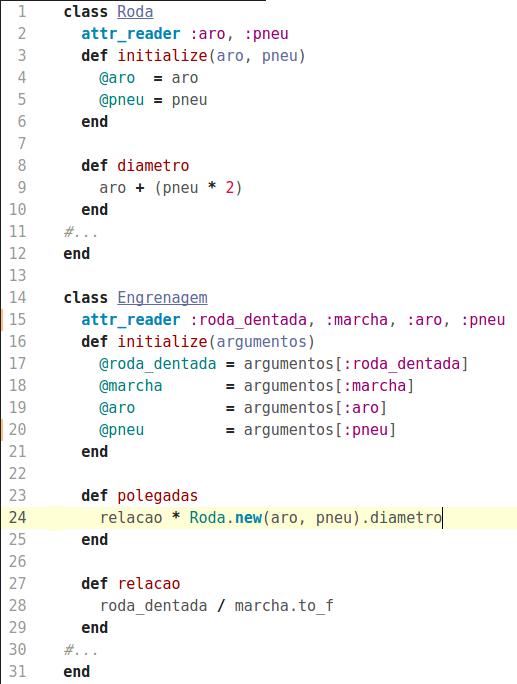
\includegraphics[scale=0.50]{imagens/codigo_pag_201.png}
  \caption{Código das Classes Roda e Engrenagem}
  \label{img:codigo_pag_201}
\end{figure}

A tabela \ref{table:mensagens} mostra as mensagens (outras além daquelas que retornam simples atributos) que cruzam os limites desses objetos. Roda responde a uma mensagem de entrada, diametro (que por sua vez é enviada por, é uma mensagem de saída de Engrenagem) e Engrenagem responde duas mensagens de entrada, polegadas e relação.
O parágrafo de abertura dessa seção dizia que toda mensagem de entrada é parte da interface pública de um objeto e portanto deve ser testada. Agora é a hora de adicionar uma pequena ressalva nessa regra.

\subsection{Apagando Interfaces Inutilizadas}

Mensagens de entrada devem ter dependentes. Como você pode ver na tabela \ref{table:mensagens}, isso é verdade para diametro, polegadas e relação onde elas são mensagens de entrada. Algum objeto além do implementador depende de cada uma dessas mensagens.
Se você desenhar essa tabela para o objeto sendo testado e encontrar uma mensagem de entrada que parece não ter dependente(s), você deve ver essa mensagem com muita suspeita. Qual é o propósito de implementar uma mensagem que ninguém envia? Ela não está chegando de forma alguma, é uma implementação especulativa que cheira a adivinhação sobre o futuro e claramente antecipa requerimentos que não existem.

Não teste mensagens de entrada que não tem dependentes, apague elas. Sua aplicação é melhorada impiedosamente ao eliminar código que não é usado. Tal código é fluxo de caixa negativo, ele adiciona o peso de testes e manutenção mas não provê valor algum. Excluir código não usado economiza dinheiro agora, se você não o apagar, você precisa testa-lo.

\begin{table}[!htbp]
  \caption{Mensagens de Entrada e Saída por Objeto}
  \label{table:mensagens}
  \centering
  \begin{tabular}{p{3.0cm} | p{3.0cm} | p{3.0cm} | p{3.0cm}}
    \toprule
    \textbf{Objeto} & \textbf{Entrada} & \textbf{Saída} & \textbf{Dependentes?} \\ \midrule
    \small{Roda} & \small{diametro} & \small{} & \small{Sim} \\ \midrule
    \small{Engrenagem} & \small{} & \small{diametro} & \small{Não} \\ \midrule
    \small{} & \small{polegadas} & \small{} & \small{Sim} \\ \midrule
    \small{} & \small{relacao} & \small{} & \small{Sim}\\
    \bottomrule
  \end{tabular}
\end{table}

Supere qualquer dificuldade que você tenha; praticar essa eliminação vai te
mostrar o valor que tem. Até que chegue o momento em que você esteja completamente
convencido da exatidão nessa estratégia, você pode ser consolar com o conhecimento
de que em uma situação extrema você pode recuperar código excluído a partir do
controle de versão. Independentemente se você faz isso com prazer ou dor, apague
o código. Código inutilizado custa mais para se manter do que para se recuperar.

\subsection{Comprovando a Interface Pública}

Mensagens de entrada são testadas ao se fazer afirmações (\textit{asserts})
sobre os valores, ou estados, que suas chamadas retornam. O primeiro
requerimento para testar uma mensagem de entrada é provar que ela retorna
o valor correto para todas as situações possíveis. O código da Figura \ref{img:codigo_pag_203}
mostra um teste do método diametro da classe Roda. A linha 4 cria uma
instância de Roda e a linha 5 afirma que o diametro dessa Roda é 29.

\begin{figure}[!htbp]
  \center
  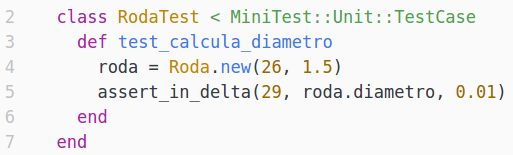
\includegraphics[scale=0.50]{imagens/codigo_pag_203.png}
  \label{img:codigo_pag_203}
\end{figure}

Esse é um teste extremamente simples e usa muito pouco código. Roda não tem
dependência alguma escondida, então nenhum outro objeto em sua aplicação é
criado como efeito colateral ao se executar esse teste. O \textit{design}
de Roda permite que você teste ela independente de todas as outras classes
em sua aplicação.

Testar Engrenagem é um pouco mais interessante. Engrenagem requer mais
alguns argumentos do que Roda, mas mesmo assim a estrutura geral desses dois
testes são muito parecidas. No teste do método polegadas na Figura \ref{img:codigo_pag_204},
a linha 4 cria uma instância de Engrenagem e a linha 10 faz afirmações sobre
os resultados do método.

\begin{figure}[!htbp]
  \center
  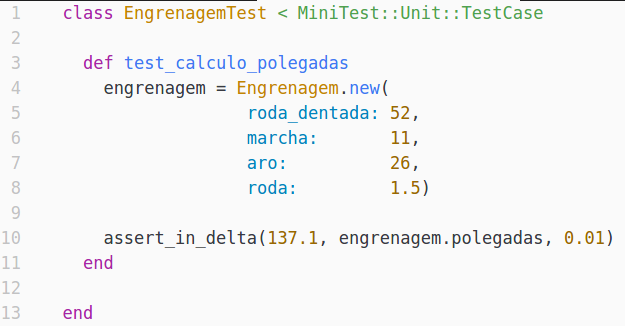
\includegraphics[scale=0.50]{imagens/codigo_pag_204.png}
  \label{img:codigo_pag_204}
\end{figure}

Esse teste de polegadas parece muito com o teste de diametro em Roda, mas não
se engane pelas aparências. Esse teste tem um emaranhamento que o teste de
diametro não tinha. A implementação do método polegadas em Engrenagem cria e
usa outro objeto incondicionalmente, Roda. Engrenagem e Roda estão acoplados em
código e nos testes, ainda que não esteja óbvio aqui.

O fato do método polegadas em Engrenagem criar e usar outro objeto afeta quanto
tempo esse teste roda e qual a probabilidade dele sofrer consequências
não intencionadas como resultado de mudanças em partes não relacionadas da
aplicação. O acoplamento é o que cria esse problema, porém, está escondido
dentro de Engrenagem e por isso totalmente invisível para esse teste. O propósito
do teste é provar que polegadas retorna o resultado correto e ele certamente cumpre
esse requerimento, mas a maneira como o código por baixo está estruturado adiciona
riscos ocultos.

Se objetos da classe Roda forem custosos para serem criados, o teste em
Engrenagem paga esse preço mesmo que ele não tenha interesse em Roda. Se
Engrenagem está correto, mas Roda está quebrada, o teste em Engrenagem pode
falhar de uma forma enganosa, em um lugar muito distante do código que você
está tentando testar.

Testes rodam o mais rápido possível quando eles executam apenas o mínimo de
código. O volume de código externo que o teste invoca está diretamente
relacionado com o seu \textit{design}. Uma aplicação construída com objetos
fortemente acoplados e carregados de dependências são como um tapete onde puxar
um dos fios arrasta o tapete inteiro. Quando objetos fortemente acoplados são
testados, o teste de um objeto roda código de muitos outros. Se o código estivesse
organizado de forma que Roda também estivesse acoplado a outros objetos, esse
problema seria ampliado. Executar o teste em Engrenagem iria então criar uma
grande rede de objetos, onde qualquer um deles poderia quebrar o teste de uma
forma enlouquecedoramente confusa.

Esses problemas são manifestados em testes, mas não são acontecem apenas neles.
Devido aos testes serem a primeira reutilização de código, esse problema é apenas um
precursor das coisas que virão para a sua aplicação como um todo.

\section{Isolando o Objeto Sendo Testando}

Engrenagem é um objeto simples, mas tentativas de testar seu método polegadas já
nos fez descobrir sua complexidade oculta. O objetivo desse teste é certificar
que as polegadas de uma engrenagem sejam calculadas corretamente, mas acontece
que executar o método polegadas depende de código em objetos além de Engrenagem.

Isso expõe um problema de \textit{design} mais amplo. Quando você não consegue
testar Engrenagem de forma isolada, isso é um mau presságio para o futuro. Essa
dificuldade para isolar Engrenagem nos testes revela que essa classe está
limitada a um contexto específico, um que impõe limitações que irão
interferir com reúso.

O capítulo 3 removeu essa dependência ao remover a criação de Roda em
Engrenagem. A Figura \ref{img:codigo_pag_205} exibe uma cópia do código que foi
responsável por essa transição. Engrenagem agora espera ser injetado com um
objeto que entende a mensagem diametro.

\begin{figure}[!htbp]
  \center
  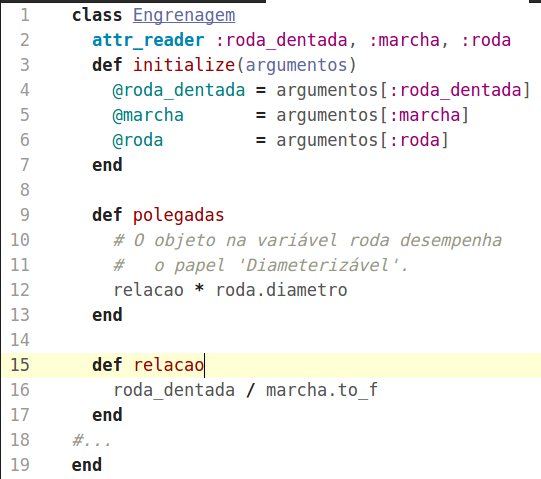
\includegraphics[scale=0.50]{imagens/codigo_pag_205.png}
  \label{img:codigo_pag_205}
\end{figure}

Essa mudança em código está relacionada a mudança de raciocínio.
Engrenagem não se importa mais com a classe do objeto injetado, ela simplesmente
espera que o objeto implemente diametro. O método diametro é parte da interface
pública de um papel (\textit{role}, em inglês), um que poderia ser chamado
razoavelmente de 'Diameterizável'.

Agora que Engrenagem está desacoplada de Roda, você deve injetar uma instância
de um Diameterizável durante a criação de toda Engrenagem. Entretanto, como
Roda é a única classe na aplicação que desempenha esse papel, suas opções em
tempo de execução estão seriamente limitadas. Na vida real, da forma como o
código está, cada Engrenagem que você criar será necessariamente injetada com uma
instância de Roda.

Apesar disso soar paradoxal, injetar uma Roda em Engrenagem não é o mesmo que
injetar um um 'Diameterizável'. O código da aplicação parece exatamente o mesmo,
admito, mas o significado lógico difere. A diferença não está nos caracteres
que você digita, mas no seu raciocínio sobre o que eles significam. Libertar sua
imaginação de um anexo em classes de objetos que virão abre possibilidades de
\textit{design} e testes que de outra forma não estariam disponíveis. Pensar no
objeto injetado como uma instância de seu papel fornece mais escolhas sobre
que tipo de 'Diameterizável' injetar em Engrenagem durante seus testes.

Uma possibilidade de 'Diameterizável' é, obviamente, Roda, porque ela claramente
implementa a interface correta. O próximo exemplo faz essa escolha banal, ele
atualiza o teste existente para acomodar as mudanças no código ao injetar uma
instância de Roda (linha 6) durante o teste.

\begin{figure}[!htbp]
  \center
  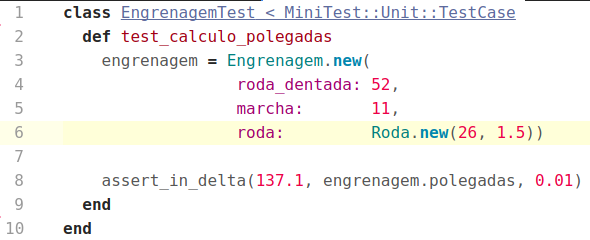
\includegraphics[scale=0.50]{imagens/codigo_pag_206.png}
  \label{img:codigo_pag_206}
\end{figure}

Usar uma Roda para o 'Diameterizável' injetado resulta em código
de teste que espelha exatamente a aplicação. Agora é óbvio,
tanto na aplicação quanto nos testes, que Engrenagem está usando
Roda. Esse acoplamento invisível entre essas classes foi exposto
publicamente.

Esse teste é rápido o suficiente, mas essa velocidade adequada é
inteiramente acidental. Não é como se o teste do cálculo de
polegadas estivesse cuidadosamente isolado e portanto
desacoplado de outro código, nem um pouco, é que apenas todo o
código acoplado nesse teste é executado rapidamente também.

Observe que não é óbvio aqui (ou em qualquer outro lugar) que Roda está
desempenhando a função de 'Diameterizável'. A função é virtual, tudo está na sua
cabeça. Nada no código guia mantenedores futuros a pensar em Roda como um
'Diameterizável'. Contudo, apesar da invisibilidade da função e esse
acomplamento a Roda, estruturar o teste dessa forma tem uma vantagem muito real,
conforme exibido na próxima seção.

\section{Injetando Dependências Usando Classes}

Quando o código em seu teste usa os mesmos objetos colaboradores que o código em
sua aplicação, seus testes sempre quebram quando eles deveriam. O valor disso
não pode ser subestimado.
Aqui está um exemplo simples. Imagine que a interface pública dos
'Diameterizáveis' mude. Outro programador vai até a classe de Roda e altera o
nome do método diametro para largura, conforme ilustrado na linha 8 abaixo.

\begin{figure}[!htbp]
  \center
  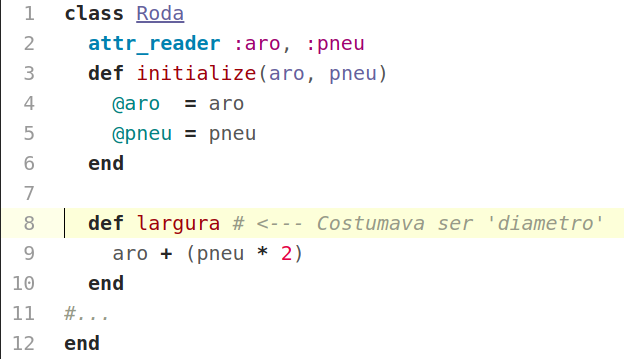
\includegraphics[scale=0.50]{imagens/codigo_pag_207_a.png}
  \label{img:codigo_pag_207_a}
\end{figure}

Imagine ainda que esse programador falhou em atualizar o nome da mensagem
enviada por Engrenagem. Engrenagem ainda envia diametro em seu método polegadas,
conforme você pode ver nesse lembrete do código atual de Engrenagem.

\begin{figure}[!htbp]
  \center
  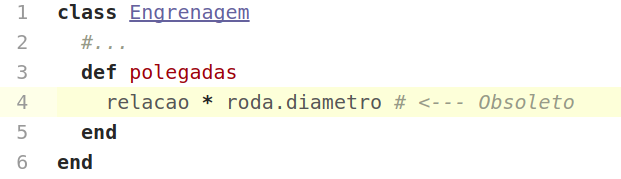
\includegraphics[scale=0.50]{imagens/codigo_pag_207_b.png}
  \label{img:codigo_pag_207_b}
\end{figure}


Porque o teste de Engrenagem injeta uma instância de Roda e Roda implementa
largura, mas Engrenagem envia diametro, o teste agora falha:

\begin{figure}[!htbp]
  \center
  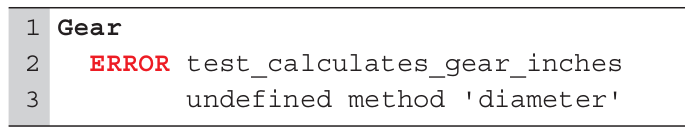
\includegraphics[scale=0.50]{imagens/codigo_pag_208_a.png}
  \label{img:codigo_pag_208_a}
\end{figure}

Essa falha não é uma surpresa, é exatamente o que deveria acontecer quando dois
objetos concretos colaboram e o destinatário da mensagem muda, mas o remetente
não. Roda mudou e como resultado Engrenagem precisa mudar. Esse teste falha como
deveria.
O teste é simples e a falha óbvia porque o código é tão concreto, mas como tudo
que é concreto ele só funciona para esse caso específico. Aqui, para esse
código, o teste acima é bom o suficiente, mas existem outras situações onde você
estaria melhor servido localizando e testando a abstração.
Um exemplo mais extremo ilumina o problema. Se existirem centenas de
'Diameterizáveis', como você decide qual revela melhor suas intenções durante os
testes? E se os 'Diameterizáveis' forem extremamente custosos, como você
evitaria executar um monte de código desnecessário e demorado? O senso comum
sugere que se Roda é o único 'Diameterizável' e ele é rápido o suficiente, o
teste deveria apenas injetar uma Roda, mas e se suas opções forem menos óbvias?

\subsection{Injetando Dependências Como Papéis}

A classe Roda e o papel 'Diameterizável' estão tão intimamente alinhadas que é
difícil ver elas como conceitos separados, mas compreender o que aconteceu no
teste anterior requer fazer a distinção. Engrenagem e Roda ambas têm relações
com uma terceira coisa, o papel 'Diameterizável'. Como você pode ver na Figura
\ref{img:codigo_pag_208_b} 'Diameterizável' é uma dependência de
Engrenagem e é implementada por Roda.

\begin{figure}[!htbp]
  \center
  \caption{Engrenagem depende de um 'Diameterizável'; Roda o implementa.}
  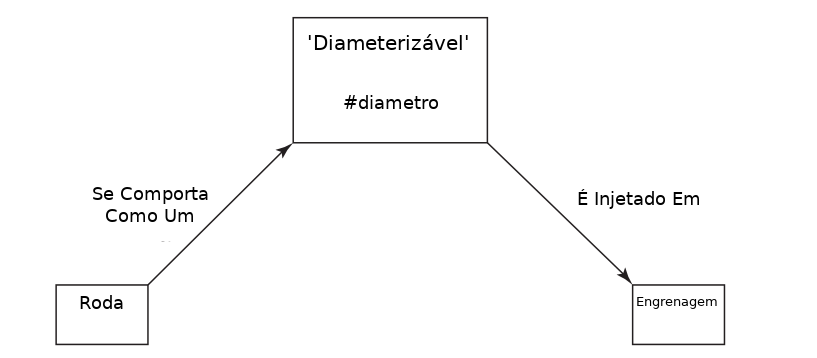
\includegraphics[scale=0.50]{imagens/codigo_pag_208_b.png}
  \label{img:codigo_pag_208_b}
\end{figure}

Esse papel é uma abstração a partir da ideia de que diferentes objetos podem ter
diâmetro. Como em todas as abstrações, é sensato esperar que esse papel abstrato
seja mais estável do que o código concreto de onde ela veio. No entanto, para
o caso específico acima, o oposto é verdade.

Existem dois lugares no código onde um objeto depende do conhecimento de
'Diameterizável'. Primeiro, Engrenagem acha que conhece a interface de
'Diameterizável', isso significa que ela acredita que pode enviar diametro para
o objeto injetado. Segundo, o código que criou o objeto para ser injetado
acredita que Roda implementa essa interface, isso significa que ela espera que
Roda implemente diametro. Agora que 'Diameterizável' mudou, existe um problema.
Roda foi atualizada para implementar a nova interface, mas infelizmente
Engrenagem ainda espera a interface antiga.

O motivo todo de injenção de dependências é que isso permite que você
substitua diferentes classes concretas sem ter que alterar código existente.
Você pode juntar comportamento novo ao criar objetos que desempenham papéis
existentes e injetar esses objetos onde esses papéis são esperados.
\textit{Design} orientado a objetos diz para você injetar dependências porque
acredita que classes específicas e concretas irão mudar mais do que esses
papéis ou, de modo inverso, papéis serão mais estáveis do que as classes de
onde foram abstraídos.

Infelizmente, o opostos acabou de acontecer. Nesse exemplo não foi a classe
do objeto injetado que mudou, foi a interface do papel. Ainda é correto injetar
uma Roda, mas agora incorreto enviar para essa Roda a mensagem diametro.

Quando um papel tem apenas um ator, esse único ator concreto e o papel abstrato
são tão estreitamente alinhados que os limites entres eles ficam facilmente
ofuscados e é um fato prático que algumas vezes esse ofuscamento não importa.
Nesse caso Roda é o único ator de 'Diameterizável' e você não espera atualmente
ter outros. Se Rodas são baratas, injetar uma Roda de verdade tem pouco efeito
negativo em nossos testes.

Quando o código da aplicação pode ser apenas escrito de um jeito, espelhar esse
arranjo é frequentemente o jeito mais eficiente de escrever testes. Fazendo
dessa forma permite que o  teste falhe corretamente independentemente de se
a concretização (o nome da classe Roda) ou a abstração (a interface do método
diametro) mudem.

No entanto, isso não é sempre verdade. Algumas vezes existem forças que te levam
a querer esquecer o uso de Roda em seus testes. Se sua aplicação contém muitos
'Diameterizáveis' diferentes você talvez queira criar um idealizado de forma que
seus testes claramente transmitam a ideia desse papel. Se todos os
'Diameterizáveis' são caros, você talvez queira falsificar um barato para fazer
seus testes serem executados mais rapidamente. Se você está fazendo BDD, sua
aplicação pode ainda não conter nenhum objeto que desempenhe esse papel, você
pode ser forçado a manufaturar algo apenas para escrever o teste.

\subsection{Criando Dublês de Teste}

Esse próximo exemplo explora a ideia de criar um objeto falso, ou dublê de
testes, para desempenhar o papel 'Diameterizável'. Para esse teste, assuma que
a interface foi revertida para o método original diametro e que diametro está
novamente sendo implementado por Roda e enviado por Engrenagem. A linha 2 na
Figura \ref{img:codigo_pag_210} cria um objeto falso, DiametroDuble.
A linha 13 injeta esse objeto falso em Engrenagem.

Um dublê de testes é uma instância estilizada de um ator de um papel
que é usado exclusivamente para testar. Dublês como esse são muito fáceis de
serem criados, nada impede você de criar um para cada situação possível. Cada
variante é como um rascunho de um artista. Ele realça uma única funcionalidade
e permite que outros detalhes sobre esse objeto fiquem para trás.

\begin{figure}[!htbp]
  \center
  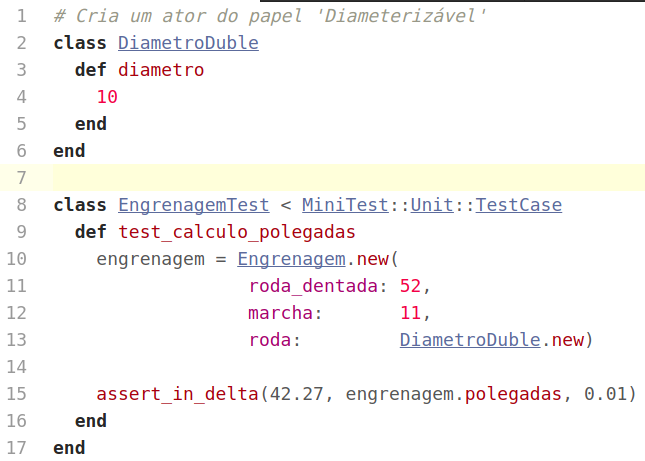
\includegraphics[scale=0.50]{imagens/codigo_pag_210.png}
  \label{img:codigo_pag_210}
\end{figure}

Esse dublê é um \textit{stub} para o método diametro, ou seja, ele implementa
uma versão de diametro que retorna uma resposta pré-determinada. DiametroDuble
é bem limitado, mas esse é o objetivo. O fato dele retornar sempre 10 para
diametro é perfeito. O valor retornado pelo \textit{stub} fornece uma fundação
confiável na qual podemos construir o teste.

Muitos \textit{frameworks} de teste possuem maneiras incorporadas para criação
de dublês e \textit{stubs}. Esses mecanismos especializados podem ser
convenientes, mas para dublês de testes simples, você pode usar objetos puros
em Ruby, como no exemplo acima.

DiametroDuble não é um \textit{mock}. É fácil acabar adquirindo o hábito de usar
a palavra "\textit{mock}" para descrever esse dublê, mas \textit{mock} é outra
coisa completamente diferente e será discutido nesse capítulo na seção
Testando Mensagens de Saída.

Injetar esse dublê desacopla o teste de Engrenagem da classe Roda. Não importa
mais se Roda é lenta, porque DiametroDuble é sempre rápido. Esse teste
funciona bem, como mostra a execução dele.

Esse teste usa um dublê de testes e assim sendo é simples, fácil, isolado e
revelador quanto as suas intenções; o que poderia possivelmente dar errado?

\subsection{Vivendo o Sonho}

Imagine agora que o código é submetido as mesmas alterações que antes:
A interface do 'Diameterizável' muda de diametro para largura e Roda é
atualizado, mas Engrenagem não é. Essa mudança mais uma vez quebra a aplicação.
Lembre-se que o teste anterior de Engrenagem (o qual injetou uma Roda ao invés
de usar um dublê) notou esse problema imediatamente e começou a falhar com um
erro de método 'diametro' não definido·

Agora que você está injetando um DiametroDuble, porém, o teste continua
passando, mesmo quando a aplicação definitivamente está quebrada. Essa aplicação
não tem possibilidade alguma de funcionar; Engrenagem envia diametro, mas Roda
implementa largura.

Você criou um universo alternativo, um no qual testes alegremente reportam que
tudo está bem, apesar do fato de que a aplicação está manifestamente incorreta.
A possibilidade de criar esse universo é o que causa algumas pessoas a advertir
que \textit{stubbing} (e \textit{mocking}) criam testes frágeis. Entretanto,
como é sempre verdadeiro, a culpa aqui é do programador e não da ferramenta.
Escrever código melhor requer a compreensão da causa raiz desse problema, o
qual, por sua vez, requer um olhar mais profundo de seus componentes.

A aplicação contém um papel chamado 'Diameterizável'. Esse papel originalmente
tinha apenas um ator, Roda. Quando o teste de Engrenagem criou DiametroDuble,
ele introduziu um segundo ator do papel. Quando a interface do papel muda,
todos os atores do papel precisam adotar a nova interface. É fácil, no entanto,
negligenciar atores que foram construídos especificamente para testes e foi
exatamente isso que aconteceu aqui. Roda foi atualizado com uma nova interface,
mas DiametroDuble não foi.

\subsection{Usando Testes Para Documentar Papéis}

Não é nenhuma surpresa que esse problema ocorra. O papel é quase invisível. Não
existe um lugar na aplicação onde você possa apontar o dedo e dizer "Isso
define um 'Diameterizável'." Quando lembrar que o papel existe é difícil,
esquecer que dublês de teste o desempenham é inevitável.

Um jeito de aumentar a visibilidade do papel é certificando-se (\textit{assert})
que Roda o desempenha. A linha 6 na Figura \ref{img:codigo_pag_211} faz
exatamente isso. Documenta o papel e prova que Roda implementa sua interface
corretamente.

\begin{figure}[!htbp]
  \center
  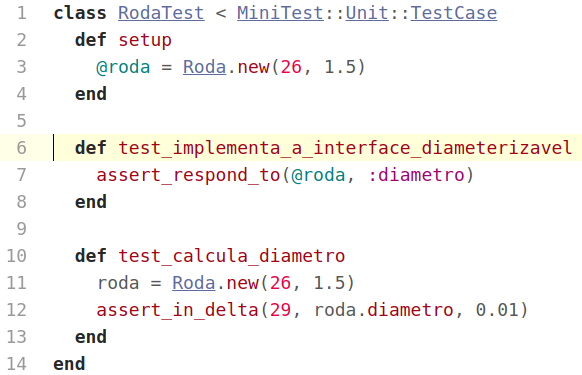
\includegraphics[scale=0.50]{imagens/codigo_pag_211.png}
  \label{img:codigo_pag_211}
\end{figure}

O teste \verb|implementa_a_interface_diameterizavel| introduz a ideia de testes
para papéis, mas não é uma solução completamente satisfatória. Ela é, na
verdade, lamentavelmente incompleta. Primeiramente, ela não pode ser
compartilhada com outros 'Diameterizáveis'. Outros atores desse papel teriam que
duplicar esse teste. Segundo, ela não faz nada para ajudar com o problema do
teste de Engrenagem citado na seção "Vivendo o Sonho". Certificar-se que Roda
desempenhe esse papel não evita que o DiametroDuble de Engrenagem fique obsoleto
e permita que o teste de polegadas passe de modo equivocado.

Felizmente, o problema de documentar e testar papéis tem uma solução simples,
uma que será completamente coberta na seção seguinte, Provando a Exatidão dos
Patos. Por agora, é suficiente apenas reconhecer que papéis precisam de testes
próprios.

O objetivo dessa seção foi provar as interfaces públicas através de testes das
mensagens de entrada. Roda foi barato de testar. O teste original de Engrenagem
foi mais caro porque dependia de um acomplamento escondido com Roda. Substituir
essa dependência por um dependência injetada de 'Diameterizável' isolou o
objeto sendo testado, mas criou um dilema sobre injetar um objeto real ou falso.

Essa escolha entre injetar um objeto falso ou real tem consequências de longo
alcance. Injetar os mesmo objetos nos testes que são usados em tempo de execução
garante que os testes quebrem corretamente, mas pode levar você a ter testes que
demoram para serem executados. De forma alternativa, injetar dublês pode
aumentar a velocidade de execução dos testes, mas deixa-los vulnerável a criação
de um mundo fantasioso onde testes funcionam, mas a aplicação falha.

Observe que o ato de testar não forçou, por si só, nenhuma melhoria de
\textit{design}. Nada sobre os testes te fez remover o acomplamento e injetar a
dependência. Enquanto é verdade que a abordagem de fora para dentro do BDD
fornece maior orientação do que a do TDD, nenhuma das práticas evitaria que um
\textit{designer} inexperiente escrevesse Roda e então deixasse a criação de
uma Roda embutida dentro de Engrenagem. Esse acoplamento não deixa os testes
impossíveis, ele só aumenta custos. Reduzir o acomplamento depende de você e
conta com sua compreensão dos princípios de \textit{design}.

\section{ Testando Métodos Privados }

Algumas vezes o objeto sendo testado envia mensagens a si mesmo. Mensagens
enviadas a si mesmo chama métodos definidos na interface privada do receptor.
Essas mensagens são como árvores proverbiais caindo em florestas vazias; elas
não existem, ao menos com relação ao que o resto da sua aplicação está
interessado. Porque envios de mensagens privadas não podem ser vistos fora da
caixa preta dos objetos sendo testados, elas não precisam ser testadas no mundo
intocado do \textit{design} idealizado.

No entanto, o mundo real não é tão arrumado e essa regra simples não satisfaz
completamente. Lidar com mensagens privadas requer julgamento e flexibilidade.

\subsection{ Ignorando Métodos Privados Durante Testes }

Existem muitas razões excelentes para se omitir testes de métodos privados.
Primeiramente, tais testes são redundantes. Métodos privados estão escondidos
dentro do objeto sendo testado e não podem ser vistos por outros. Esses métodos
são chamados por métodos públicos que já possuem testes. Um bug em um método
privado pode certamente quebrar a aplicação no geral, mas essa falha sempre será
exposta por um teste existente. Testar métodos privados nunca é necessário.

Segundo, métodos privados são instáveis. Testes de métodos privados estão
portanto acoplados a códigos da aplicação que são prováveis de mudarem. Quando a
aplicação muda os testes são forçados a mudar por sua vez. É fácil criar uma
situação onde tempo precioso é gasto executando manutenção de testes
desnecessários.

Finalmente, testes de métodos privados pode induzir outros a usa-los. Testes
fornecem documentação sobre o objeto sendo testado. Eles irão contar uma
história sobre como ele espera interagir com o mundo em geral. Incluir métodos
privados nessa história distrai os leitores de seu principal propósito e os
encoraja a quebrar o encapsulamento e depender nesses métodos. Seus testes
deveriam esconder métodos privados, não os expor.

\subsection{ Removendo Métodos Privados da Classe Sendo Testada }

Uma maneira de contornar esse problema inteiro é evitar métodos privados de modo
geral. Se você não tem métodos privados, você não precisa se preocupar com os
testes deles.

Um objeto com muitos métodos privados exala o cheiro de um \textit{design} que
tem muitas responsabilidades. Se seu objeto tem tantos métodos privados que você
não ousa deixa-los sem testes, considere a extração desses métodos em um novo
objeto. Os métodos extraídos formam as responsabilidades centrais do novo
objeto e portanto fazem parte da interface pública dele, a qual é
(teoricamente) estável e assim seguro de depender nela.

Essa estratégia é boa, mas infelizmente só é verdadeiramente útil se a nova
interface for realmente estável. Algumas vezes a nova interface não é, e é nessa
parte que teoria e prática se separam. Essa nova interface pública será
exatamente tão estável (ou instável) quanto a interface privada original.
Métodos não se tornam magicamente mais confiáveis apenas porque foram movidos.
É custoso se acoplar a métodos instáveis, independemente se eles são
representados como públicos ou privados.

\subsection{ Escolhendo Testar um Método Privado }

Tempos de grandes incertezas exigem medidas drásticas. Assim sendo de vez em
quando é justíficavel exalar um pouco de código com mau cheiro e esconder a
bagunça até que informações melhores cheguem. Esconder bagunças é feito
facilmente; apenas envolva o código ofensivo em um método privado.

Se você criar uma bagunça e nunca conserta-la, seus custos eventualmente irão
subir, mas a curto prazo, para o problema certo, tendo confiança suficiente para
escrever código vergonhoso pode economizar dinheiro. Quando sua intenção é adiar
uma escolha de \textit{design}, faça o que for mais simples para resolver o
problema de hoje. Isole o código atrás da melhor interface que você puder
conceber e sente e espere por mais informações.

Aplicar essa estratégia pode resultar em métodos privados que são
descontroladamente instáveis. Depois que você deu esse pulo, é razoável que
você considere ajustar seu pecados ao testar esse métodos instáveis. O
código da aplicação é feio e irá sofrer mudanças frequentes. O risco de quebrar
algo estará sempre presente. Esses testes serão custosos e provavelmente serão
forçados a mudar em conjunto com o código subjacente, mas qualquer outras opções
para manter as coisas funcionando possivelmente serão mais caras.

Esses testes de métodos privados não são necessários para se saber que uma
mudança quebrou algo. Os testes das interfaces públicas ainda servem esse
propósito de forma admirável. Testes de método privados produzem mensagens de
erros que localizam com precisão as partes do código privado que estão falhando.
Esses erros mais específicos geram acomplamentos fortes que aumentam os custos
de manutenção, mas eles tornam mais fácil compreender os efeitos das mudanças e
dessa forma eles removem parte da dor de reforatorar código privado complexo.

Reduzir as barreiras para refatoração é importante, porque refatorar você irá.
Esse é o objetivo final. A bagunça é temporária, você pretende refatorar e se
livrar dela. Como mais informações de \textit{design} chegarão, esse métodos
privados irão melhorar. Uma vez que a neblina suma e um \textit{design} se
revele, os métodos se tornarão mais estáveis. Conforme a estabilidade aumenta,
o custo da manutenção e a necessidade para os testes irão diminuir.
Eventualmente será possível extrair os métodos privados em uma classe separada
e revelar eles para o mundo.

As regras de ouro para testes de métodos privados são estas: Nunca os escreva, e
se você o fizer, jamais os teste, a menos, claro, que isso faça sentido.
Assim sendo, esteja inclinado contra escrever esses testes, mas não tenha medo
de o fazer se isso melhorar a sua parte.

\subsection{ Testando Mensagens de Saída }

Mensagens de saída, como você sabe da seção "O que Testar", são ou consultas
(\textit{queries}) ou comandos. Mensagens de consulta são importantes apenas
para o objeto que as envia, enquanto mensagens de comando têm efeitos que são
visíveis para outros objetos na sua aplicação.

\subsection{ Ignorando Mensagens de Consulta }

Mensagens que não têm efeitos colaterais são conhecidas como mensagens de
consulta. Aqui está um exemplo simples, onde o método polegadas de Engrenagem
envia a mensagem diametro.

\begin{figure}[!htbp]
  \center
  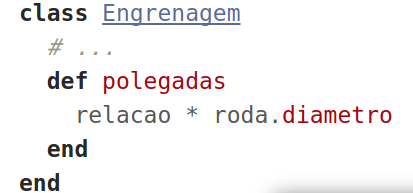
\includegraphics[scale=0.50]{imagens/codigo_pag_215.png}
  \label{img:codigo_pag_215}
\end{figure}

Nada na aplicação, além do método polegadas, se importa que a mensagem diametro seja enviada. O método diametro não tem efeitos colaterais, executar essa função não deixa nenhum rastro visível e nenhum outro objeto depende em sua execução.

Da mesma forma que testes deveriam ignorar mensagens enviadas para si mesmo (self), eles também deveriam ignorar mensagem de consulta (query). As consequências de enviar a mensagem diametro estão escondidas dentro de Engrenagem. Porque a aplicação, no geral, não precisa que esssa mensagem seja enviada, seus testes não precisam se importar.

O método polegadas de Engrenagem depende do resultado que o método diametro retorna, mas os testes que provam que essa função está correta pertencem a classe Roda, não aqui na classe Engrenagem. É redundante para Engrenagem duplicar esses testes, o custo de manutenção vai aumentar se ele o fizer. A única responsabilidade de Engrenagem é provar que polegadas funciona corretamente e isso pode ser feito simplesmente testando que polegadas sempre retorna os resultados apropriados.

\subsection{ Provando Mensagens de Comando }

Algumas vezes, no entanto, é importante que uma mensagem seja enviada, outras partes da sua aplicação dependem de alguma coisa que acontece como resultado. Nesse caso, o objeto sendo testado é responsável por enviar a mensagem e seus testes precisam provar que ele o faz.

Ilustrar esse problema requer um exemplo novo. Imagine um jogo onde jogadores correm com bicicletas virtuais. Essas bicicletas, evidentemente, possuem engrenagens. A classe Engrenagem agora é responsável por deixar a aplicação sabendo quando o jogador troca de marcha, de forma que o restante da aplicação possa atualizar o comportamente da bicicleta.

No código seguinte, Engrenagem recebe esse novo requisito ao adicionar um observador (observer). Quando um jogador trocar de marcha, os métodos estabelecer marcha e estabelecer roda dentada são executados. Esses métodos salvam o novo valor e chamam a função mudou (linha 20). Esse método então envia a mensagem mudou para o observador, passando a marcha e roda dentada atuais como parâmetros.

\begin{figure}[!htbp]
  \center
  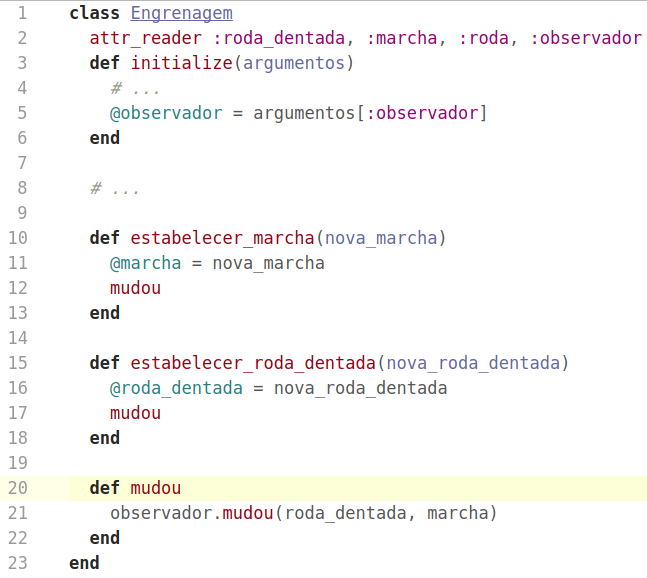
\includegraphics[scale=0.50]{imagens/codigo_pag_216.png}
  \label{img:codigo_pag_216}
\end{figure}

Engrenagem tem uma nova responsabilidade. Ela precisa notificar observador quando \underline{marcha} e \underline{roda dentada} mudarem. Essa nova responsabilidade é tão importante quanto sua obrigação anterior de calcular \underline{polegadas}. Quando um jogador trocar de marcha, a aplicação só vai estar correta se Engrenagem enviar a mensagem \underline{mudou} para \underline{observador}. Seus testes deveriam provar que essa mensagem é enviada.

Eles não deveriam apenas provar isso, mas eles também deveriam fazer isso sem afirmar (\textit{assert}) nada sobre o resultado de retorno do método \underline{mudou} de \underline{observador}. Assim como os testes de Roda alegaram serem os únicos responsáveis por fazer afirmações sobre os resultados de seus próprios métodos, os testes de \underline{observador} são os únicos que devem fazer afirmações sobre os resultados de seu método \underline{mudou}. A responsabilidade de testar o valor de retorno de uma mensagem existe apenas no receptor. Adicionar essa responsabilidade em qualquer outro lugar duplica os testes e aumenta os custos.

Para evitar duplicações você precisa de um jeito de provar que Engrenagem envia a mensagem \underline{mudou} para \underline{observador} de uma forma que não te faça depender de ter que checar o que é retornado quando a mensagem for enviada.  Felizmente, isso é fácil, você precisa de uma imitação (\textit{mock}). \textit{Mocks} são testes de comportamento, o oposto de testes de estado. Ao invés de fazer afirmações sobre o retorno de uma mensagem, \textit{mocks} definem uma expectativa de que a mensagem será enviada.

O teste abaixo prova que Engrenagem cumpre suas responsabilidades e o teste faz isso sem ficar acomplado aos detalhes de como \underline{observador} se comporta. O teste cria um \textit{mock} (linha 4) que é injetado no lugar do \underline{observador} (linha 8). Cada método do teste diz ao \textit{mock} para esperar o recebimento da mensagem \underline{mudou} (linhas 12 e 17) e então verifica que isso aconteceu (linhas 14 e 20).
